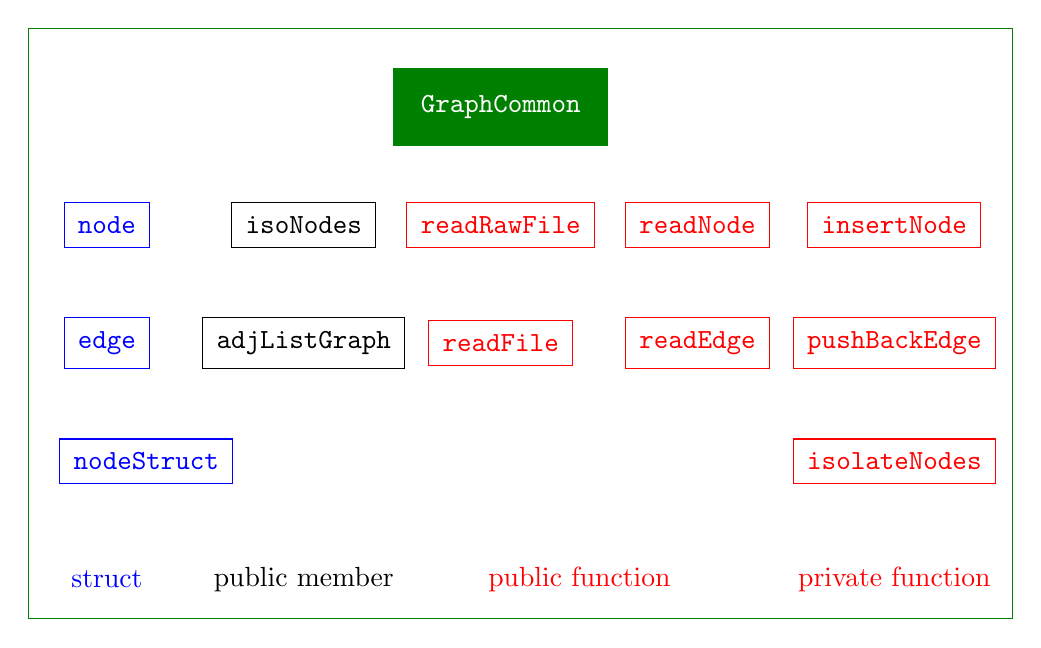
\begin{tikzpicture}
\tikzstyle{class} = [font=\ttfamily\bfseries,color=white,fill=green!50!black,inner sep=10];
\tikzstyle{struct} = [font=\ttfamily\bfseries,color=blue,draw=blue, inner sep = 5];
\tikzstyle{member} = [font=\ttfamily,draw, inner sep=5]
\tikzstyle{function} = [font=\ttfamily\bfseries,color=red,draw=red, inner sep = 5];
\node [class] at (-2,3.5) {GraphCommon};
\node [struct] at (-7,2) {node};
\node [struct] at (-7,0.5) {edge};
\node [struct] at (-6.5,-1) {nodeStruct};
\node [member] at (-4.5,2) {isoNodes};
\node [member] at (-4.5,0.5) {adjListGraph};
\node [function] at (-2,0.5) {readFile};
\node [function] at (-2,2) {readRawFile};
\node [function] at (0.5,2) {readNode};
\node [function] at (0.5,0.5) {readEdge};
\node [function] at (3,2) {insertNode};
\node [function] at (3,0.5) {pushBackEdge};
\node [function] at (3,-1) {isolateNodes};
\draw [green!50!black]  (-8,4.5) rectangle (4.5,-3);
\node [blue] at (-7,-2.5) {struct};
\node at (-4.5,-2.5) {public member};
\node [red] at (-1,-2.5) {public function};
\node [red] at (3,-2.5) {private function};
\end{tikzpicture}